\documentclass{beamer}

\usepackage[style=numeric,maxnames=2]{biblatex}
\usepackage{minted}
\usepackage{tikz}

\definecolor{lightgray}{gray}{0.9}
\definecolor{mediumslateblue}{HTML}{7B68EE}
\newcommand*\circled[1]{\tikz[baseline=(char.base)]{\node[shape=circle,fill,inner sep=2pt] (char) {\textcolor{white}{#1}};}} % chktex 36

\usepackage[orientation=portrait,size=a1,scale=1.0]{beamerposter}
\usetheme{JuelichPoster}

\ExecuteBibliographyOptions{%
  sorting=nyt,
  bibwarn=true,
  isbn=false, %keine isbn anzeigen
  url=true %keine url anzeigen
}
\addbibresource{references.bib}

\setbeamertemplate{partner1}{
\includegraphics{img/cscs}}
\setbeamertemplate{partner2}{
\includegraphics{HBP_logo.jpg}}
% TODO Add HBP and/or eBrains here

\begin{document}
\begin{frame}[t, fragile]
  \frametitle{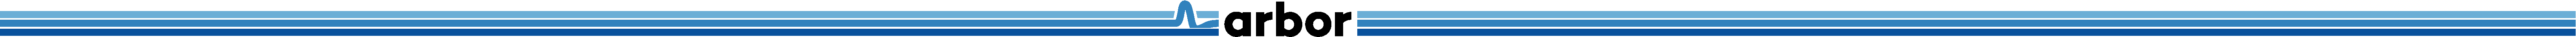
\includegraphics[width=0.66\linewidth]{img/arbor-lines-proto-colour-full}}
  \framesubtitle{A morphologically detailed neural network simulation library for modern high performance computer architectures.\\
    \tiny{Nora Abi Akar, Ben Cumming, Stuart Yates (CSCS); Thorsten Hater, Brent Huisman, Anne Küsters (FZJ)}}

  \begin{columns}[onlytextwidth,T]
    \begin{column}{0.65\textwidth}
      We present recent developments in Arbor, a library for the simulation of
      morphologically detailled neurons and networks thereof~\cite{arbor}. Arbor
      places strong emphasis on performance, portability, and usability. It can
      exploit modern architectures based on super-scalar multi-core processors
      and GPU accelerators. We showcase some of the features added to Arbor
      since the last release and how they can used to almost directly import and
      run single cell models from the Allen Brain Atlas database. These are
      interesting, non-trivial models on their own, but more importantly form
      the basis for a set of models for the mouse primary visual cortex
      network~\cite{allen-v1}.
    \end{column}
    \begin{column}{0.3\textwidth}
      \begin{block}{Where to find us}
        \begin{description}
          \item[Contact] arbor-sim@fz-juelich.de
          \item[Source code] github.com/arbor-sim/arbor
          \item[Documentation] arbor.readthedocs.io
          \item[Website] arbor-sim.github.io
        \end{description}
      \end{block}
    \end{column}
  \end{columns}
  \vspace*{-2ex}
  \textbf{{\large\structure{New Features}}}\\

  \textbf{\structure{Morphology}}\\
      Arbor provides a domain specific language (DSL) for describing regions and locations on morphologies, and a dictionary for associating these descriptions with a string label. The labels are used to refer to regions and locations when setting cell properties and attributes. For example, the membrane capacitance on a region of the cell membrane, or the location of synapse instances.
      \newline

      \begin{columns}[onlytextwidth,T]

        \begin{column}{0.33\textwidth}
          \circled{1} We're loading a 10 segment cell from an \emph{.swc} file. In this file, segments are tagged 1, 2 or 3, which correspond the soma (red), an axon (grey) and a dendrite (blue). We label these regions as follows:
\begin{minted}[bgcolor=lightgray,breaklines]{python}
labels = arb.label_dict({
'soma': '(tag 1)',
'axon': '(tag 2)',
'dend': '(tag 3)'})
\end{minted}
          \begin{center}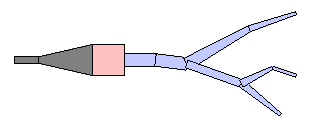
\includegraphics[width=0.8\linewidth]{scripts/morph.pdf}\end{center}
        \end{column}

        \begin{column}{0.33\textwidth}
          \circled{2} Arbor will keep number the branches of the cells automatically. In Arbor a branch is a region between branching points, starting at the proximal point {\color{red}\circled{-}} of the first segment (usually the soma). For this cell, Arbor generates {\color{mediumslateblue}\circled{6}} branches.

          In this cell, branch 1 tapers from 0.4 to 0.2 $\mu$m and branch 2 has a constant radius of 0.5 $\mu$m. Let's take two points {\color{black}\circled{-}} on the dendrite: one 80\% along branch 1 and the other 30\% along branch 2.
          \begin{center}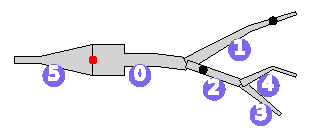
\includegraphics[width=0.8\linewidth]{scripts/branches.pdf}\end{center}
        \end{column}

        \begin{column}{0.3\textwidth}
          \circled{3} The two points and the proximal point of the soma constrain an interval where we want to place specific dynamics. We can access this region by adding a new label:
\begin{minted}[bgcolor=lightgray,breaklines]{python}
labels['roi'] = '(proximal_interval (sum (location 1 0.8) (location 2 0.3)))'
\end{minted}
          Later, we instruct Arbor to 'paint' Hodgkin–Huxley dynamics on the 'roi' regio:
\begin{minted}[bgcolor=lightgray,breaklines]{python}
cell.paint('roi', 'hh')
\end{minted}
          \begin{center}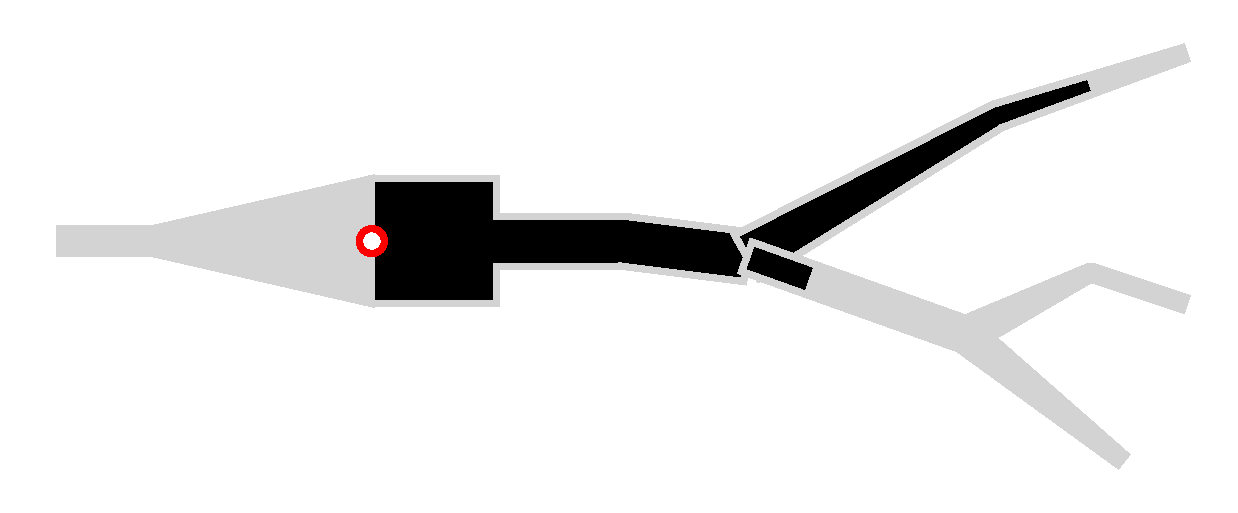
\includegraphics[width=0.8\linewidth]{scripts/region.pdf}\end{center}
        \end{column}

      \end{columns}

  \begin{columns}[onlytextwidth,T]
    \begin{column}{.49\linewidth}
      \textbf{\structure{Mechanism Catalogues}}\\
      We provide an interface to collections of \emph{mechanisms} which describe
      processes both associated with an area density like ion channels and
      localised like synapses. These mechanisms are described in the NMODL DSL
      and translated into plain or vectorised C++ and CUDA for execution on GPUs.

      In particular we currently offer two catalogues, one, called
      \emph{default} comprising basic functionality, e.g.\ a passive leak and
      secondly the \emph{allen} catalogue which is a collection of mechanisms
      obtained from the Brain Atlas\cite{mouse-atlas}. We have carefully
      optimised these, as they form the basis for the V1 network model, which is
      quite resource intensive. Catalogues are built at compile time and can be
      accessed in the simulation to provide the mechanisms used in the
      respective model. Further, they can be composed into larger catalogues,
      where name clashes are avoided via an
      optional prefix.
    \end{column}
    \begin{column}{.49\linewidth}
      \textbf{\structure{Spherical Somata}}\\
      A common pattern appearing in SWC files is the appearance of a soma
      consisting of a single point only. Up to the recent version, Arbor treated
      these as sphere with the given radius. However, it is not possible to
      resolve various ambiguities, e.g.\ where apical dendrites should be
      attached. Consequently, the interpretation of single point somata has been
      changed to a cylinder with the same surface area --- excluding caps --- as
      the sphere with the given radius. As cable segments might no longer attach
      directly to the surface, support for these detached segments was added. As
      a by-product, this change significantly simplified the associated program
      code. We offer specialised loaders for different flavours of SWC with
      clear semantics for handling the soma.
    \end{column}\\[2.5ex]
  \end{columns}
  \textbf{{\large\structure{Running an Allen Brain Atlas Model}}}\\
  The code snippet on the right is complete except the parsing and plotting
  steps; it is available in full together with this poster~\cite{my-source}.
  While the electro-physiological data is supplied as a JSON file for all
  models, the structure has some variation, precluding standardised setup.
  \begin{columns}[T]
    \begin{column}{.49\linewidth}
      \begin{itemize}
        \item[\circled{1}] load SWC structure from the download
        \item[\circled{2}] assign labels to geometry
        \item[\circled{3}] build a cell description from labels and geometry
        \item[\circled{4}] parse the electro-physiological properties supplied in the download and assign to regions
        \begin{itemize}
          \item set physical properties: $T$, $V_{m}$, $R_{a}$, $C_{m}$
          \item define ion dynamics and reversal potentials
        \end{itemize}
        \item[\circled{5}] Attach to the soma's center
        \begin{itemize}
          \item current clamp; rectangular stimulus of $150\,pA$ from $200\,ms$ to $1200\,ms$
          \item spike detector; triggering at $V=-40\,mV$
          \item voltage probe; sampling with $200\,kHz$
          %\footnote{This is added to %NB: this screws up layout big time :(
          %  the simulation, as it is a passive measurement device. Both spike
          %  current clamps and detectors (via emitting events) potentially
          %  change the model evolution.}
        \end{itemize}
        \item[\circled{6}] convert the cell description into a runnable simulation
        \item[\circled{7}] set mechanism catalogue comprising the defaults and Allen DB mechanisms.
        \item[\circled{8}] run the simulation for $1400\,ms$ with time step $\Delta t = 0.005\,ms$
      \end{itemize}
      \begin{figure}[H]
        \centering
        \includegraphics{src/arbor.pdf}
      \end{figure}
      The reference solution was obtained using the allensdk Python package with
      the default Neuron backend~\cite{neuron}. A minor modification
      was made to suppress editing of the axon at load time of the geometric
      information. For comparable simulations, we instead performed this
      manipulation by hand once and stored the result in the SWC input. We
      observe a minor deviation from the reference run, which is explained by
      different discretisations.

      The elapsed wall clock times for only the simulation steps are $14.7\,s$
      with the code on the right and $121.8\,s$ for the reference solution;
      yielding a speed-up of $8.25\times$ when using Arbor.
    \end{column}
    \begin{column}{.49\linewidth}
      \inputminted[bgcolor=lightgray,escapeinside=!!]{python}{src/model.py}
    \end{column}
  \end{columns}
%   \vspace*{2.5ex}
  \begin{columns}[T]
    \begin{column}{.49\linewidth}
      \textbf{\structure{Conclusion and Outlook}}\\
      The status quo shows that Arbor is a capable, ergonomic and highly
      performant tool for building simulations of bio-physically detailled
      neurons.

      We are working actively to further improve Arbor:
      \begin{itemize}
        \item support for computation of local field potentials (LFP)
        \item coupling with other simulators such as Nest
        \item support for NeuroML and Neurolucida cell descriptions
        \item streamlined NMODL mechanism integration without re-compilation
      \end{itemize}
    \end{column}
    \begin{column}{.49\linewidth}
      \textbf{\structure{References}}\\
      \printbibliography{}
    \end{column}
  \end{columns}

      \textbf{\structure{Acknowledgements}}\\
      This research has received funding from the European Union's Horizon 2020
      Framework Programme for Research and Innovation under the Specific Grant
      Agreements No.\,720270 (HBP SGA1), No.\,785907 (HBP SGA2), and No.\,945539
      (HBP SGA3).\\[1.5ex]
\end{frame}
\end{document}
